El firewall de SME server es modificado automáticamente en respuesta a los cambios que hacemos en la configuración, como activar o desactivar servicios, hacerlos públicos o privados o reenviar puertos.\\

Por ejemplo, si añadimos una regla de reenvío de puertos en la interfaz web:

\begin{figure}[H]
    \centering
    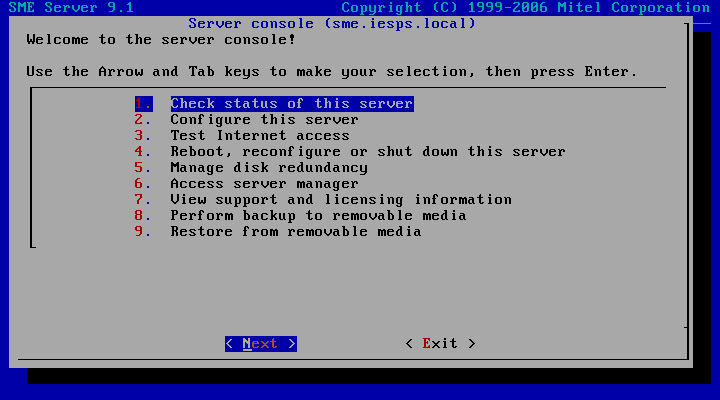
\includegraphics[width=\textwidth]{firewall/00.png}
\end{figure}

Podemos ver cómo la regla se ha añadido a la tabla \textit{nat}.

\begin{figure}[H]
    \centering
    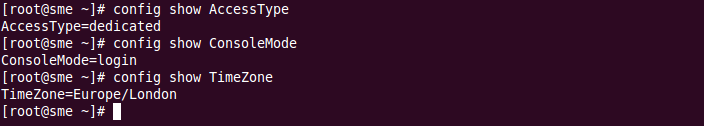
\includegraphics[width=\textwidth]{firewall/01.png}
\end{figure}

Primero consultamos la cadena PREROUTING de la tabla \textit{nat}, que es donde se tienen que añadir las reglas de Iptables para traducción de direcciones. Vemos que hay un target de nombre PortForwarding. Al no ser un target estándar de Iptables, se refiere a una cadena personalizada que el servidor ha creado. Como no tiene filtro, todos los paquetes serán pasados por esa cadena. La consultamos y vemos que a todos los paquetes que entren con IP destino 10.0.2.15 (la externa del servidor), les aplicará el target PortForwarding\_3233, que es otra cadena personalizada. Finalmente consultamos esta y vemos que está la regla que hace DNAT (en este caso se refiere a Destination NAT, cambio de la dirección de destino).\\

Hay dos formas en las que podemos hacer una configuración más avanzada del firewall: modificando ciertos valores en la base de datos para los distintos servicios o creando templates propias para cambiar directamente la configuración de Iptables.

\section{Modificación del firewall}

El archivo responsable de cargar toda la configuración de Iptables en el sistema es \lstinline!/etc/rc.d/init.d/masq!, por tanto las plantillas se encuentran en \lstinline!/etc/e-smith/templates/etc/rc.d/init.d/masq!.

\begin{figure}[H]
    \centering
    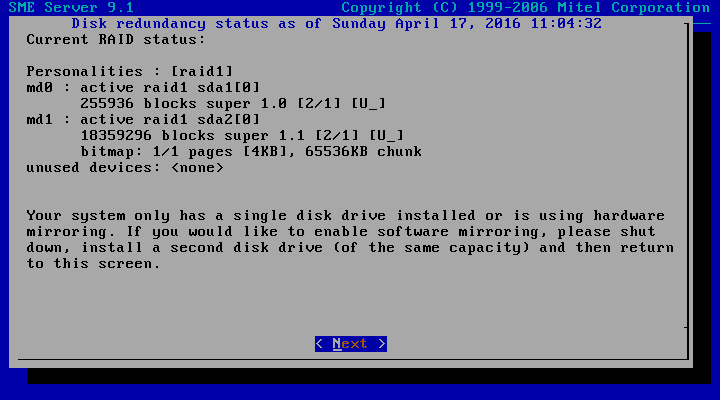
\includegraphics[width=\textwidth]{firewall/05.png}
\end{figure}

Tendremos que copiar y modificar la plantilla adecuada en \lstinline!templates-custom!, o crear una nueva, y luego expandirla con \lstinline!expand-template! y reiniciar el servicio: \lstinline!/etc/init.d/masq restart!. \\

Vamos a configurar el firewall del servidor para proporcionar una seguridad más fuerte en el caso de algunos ataques comunes:

\subsection{Denegación de servicio}

Un ataque de denegación de servicio (denial-of-service, DoS) causa que un servicio o recurso sea inaccesible a sus usuarios. Se suelen generar mediante la saturación de los puertos con flujo de información, consumiendo todo el ancho de banda y bloqueando así el servidor. Existen diferentes tipos de ataques de denegación de servicio por lo que hay que elaborar una respuesta para cada uno de ellos.\\

\begin{itemize}
\item \textbf{Ping flood}
\end{itemize}

Consiste en saturar al servidor con paquetes ICMP, enviándolos lo más rápido posible sin esperar respuesta. Esto provoca que se consuma mucho ancho de banda de entrada y también de salida, puesto que el servidor intentará responder. Es más efectivo si el ancho de banda disponible para el atacante es mayor que el del servidor.\\

Para comprobar si SME server está configurado contra el ping flood por defecto, le he cambiado el adaptador en VirtualBox a modo bridge, para que la interfaz externa esté en la misma red que mi ordenador (la nueva IP es 192.168.1.250), y le he atacado desde ahí. Todos los pings son satisfactorios con lo que SME no está protegido contra esto.

\begin{figure}[H]
    \centering
    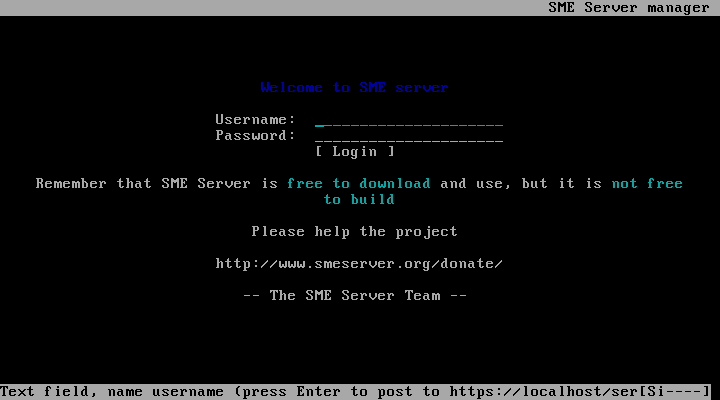
\includegraphics[width=\textwidth]{firewall/07.png}
\end{figure}

Una solución para evitar esto es permitir solamente un ping por segundo. Podemos escribir una nueva cadena para controlar esto y llamarla desde INPUT cuando se encuentren paquetes ICMP.

\begin{lstlisting}
/sbin/iptables -N icmpFlood
/sbin/iptables -A icmpFlood -p icmp --icmp-type echo-request -m limit --limit 1/s --limit-burst 1 -j ACCEPT
/sbin/iptables -A icmpFlood -j DROP

/sbin/iptables -A INPUT -p icmp -j icmpFlood
\end{lstlisting}

En este caso usaré la plantilla 39misReglas, para que la regla que está en la cadena INPUT se añada al principio. Las cadenas en la tabla \textit{filter} quedan así:

\begin{figure}[H]
    \centering
    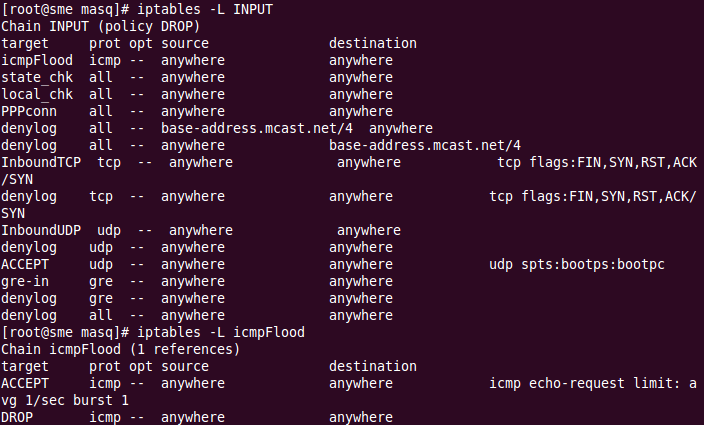
\includegraphics[width=\textwidth]{firewall/17.png}
\end{figure}

Con estas reglas se soluciona el problema. Este es el resultado al volver a intentar el ping flood desde nuestro ordenador:

\begin{figure}[H]
    \centering
    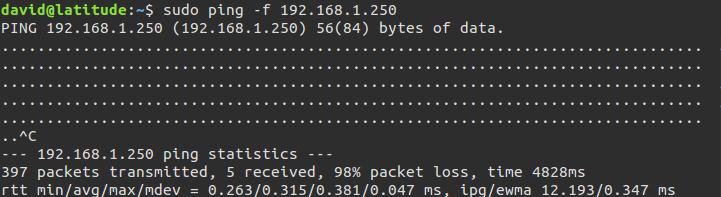
\includegraphics[width=\textwidth]{firewall/13buena.png}
\end{figure}
\vspace{0.15cm}
\begin{itemize}
\item \textbf{SYN flood}
\end{itemize}

Cuando queremos iniciar una conexión TCP, se produce el saludo a tres vías: el cliente envía un mensaje con la bandera SYN, el servidor responde con un mensaje SYN-ACK y finalmente el cliente responde con un mensaje ACK. El ataque SYN flood consiste en saturar el servidor mandando mensajes SYN y no respondiendo con los correspondientes ACK.\\

En Linux podemos usar el programa hping3 con este fin.

\begin{figure}[H]
    \centering
    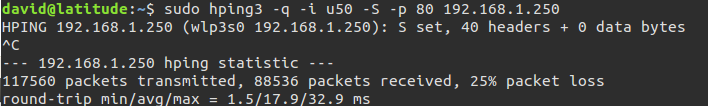
\includegraphics[width=\textwidth]{firewall/16syn.png}
\end{figure}

Con el comando de la imagen enviamos un mensaje con la bandera SYN al puerto 80 cada 50 microsegundos. Como resultado, mientras se está ejecutando este comando el servidor está bloqueado, impidiéndonos por ejemplo acceder a la interfaz web de administración.\\

Para solucionarlo de una forma distinta al anterior, se puede utilizar el módulo \lstinline!recent!:

\begin{lstlisting}
modprobe ipt_recent

/sbin/iptables -N synFlood
/sbin/iptables -A synFlood -m recent --set
/sbin/iptables -A synFlood -m recent --update --seconds 2 --hitcount 20 -j DROP

/sbin/iptables -A INPUT -p tcp --tcp-flags SYN SYN -j synFlood
\end{lstlisting}

La primera línea es para cargar el módulo. La última es para que los paquetes que tengan al menos la bandera SYN pasen por nuestra cadena synFlood. La primera regla de la nueva cadena añade la IP de origen del paquete a la lista. Si ya está en la lista, actualiza la entrada. La siguiente línea se encarga de actualizar el tiempo en el que se ha visto esa IP y rechazar los paquetes si la IP ha sido vista en la tabla en los últimos dos segundos y si tiene al menos 20 paquetes enviados. La lista que guarda los paquetes enviados no tiene en cuenta el tiempo en el que han llegado. Esto quiere decir que el control solo se reiniciará cuando la IP de origen haya estado 2 segundos sin enviar ningún paquete, o al menos ninún paquete que se haya comparado contra esta regla. Como podemos ver, ahora solo llegan 19 paquetes de vuelta:

\begin{figure}[H]
    \centering
    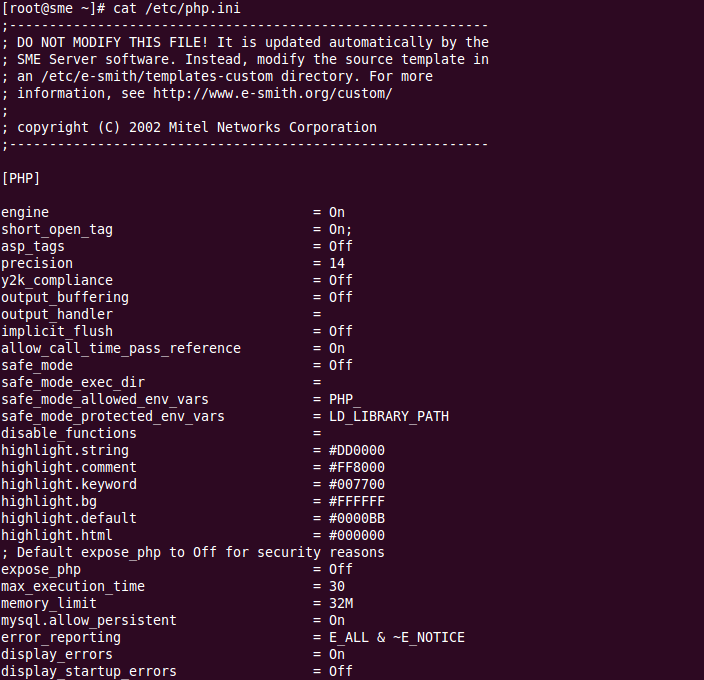
\includegraphics[width=\textwidth]{firewall/18.png}
\end{figure}

\subsection{Suplantación de identidad}

Este tipo de ataque consiste en que un host o aplicación se hace pasar por otro. Por ejemplo, nos pueden llegar paquetes desde la interfaz externa con IPs de nuestra red interna. En estos casos el atacante no se preocupa de la respuesta que origina el paquete ya que no le llegará.\\

Podemos lanzar un ataque SYN flood de manera que cada paquete que enviemos se envíe con una dirección IP de origen aleatoria, con lo que la regla que hemos creado contra estos ataques no serviría para nada. El programa hping3 permite hacerlo de manera sencilla, sin más que añadir la opción \lstinline!--rand-source!:

\begin{figure}[H]
    \centering
    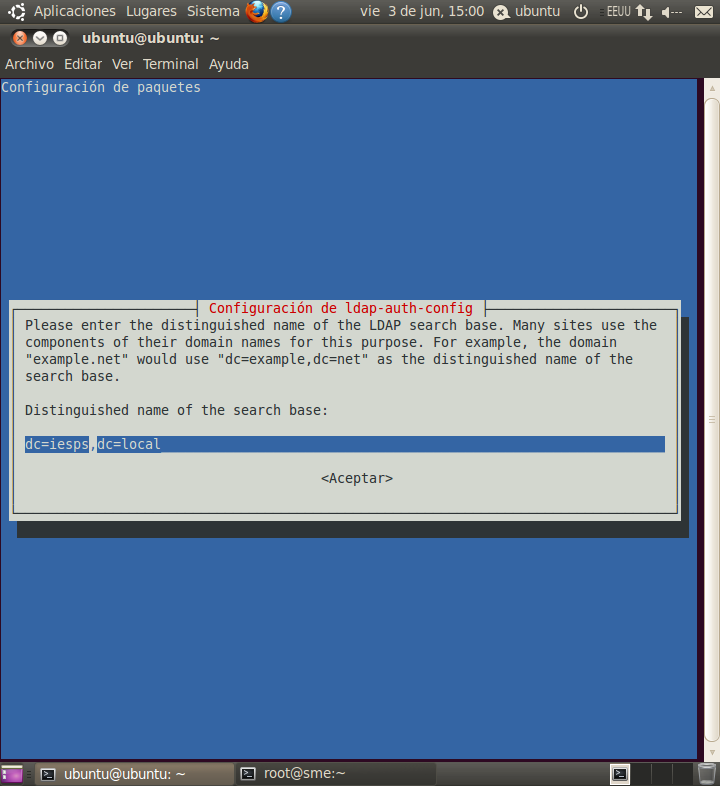
\includegraphics[width=\textwidth]{firewall/21.png}
\end{figure}

Estamos provocando que nuestro servidor mande mensajes SYN-ACK a esas IPs aleatorias.

\begin{figure}[H]
    \centering
    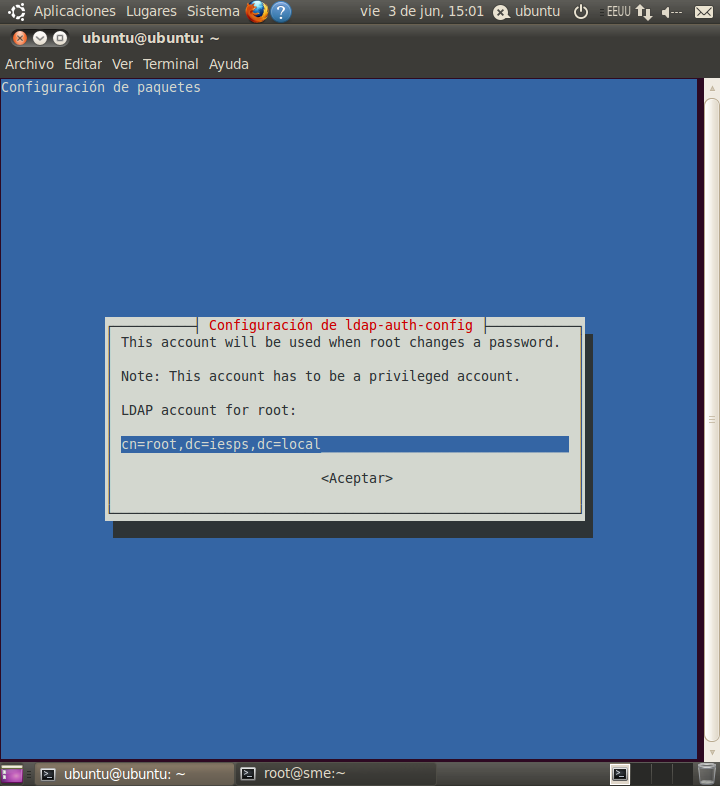
\includegraphics[width=\textwidth]{firewall/22.png}
\end{figure}

\newpage

Esto puede ser evitado con una regla de las del primer tipo, la que vimos para el ping flood.

\begin{lstlisting}
/sbin/iptables -N synFlood2
/sbin/iptables -A synFlood2 -m limit --limit 1/s --limit-burst 1 -j RETURN
/sbin/iptables -A synFlood2 -j DROP

/sbin/iptables -A INPUT -p tcp --tcp-flags SYN SYN -j synFlood2

/sbin/iptables -A INPUT -s 10.0.0.0/8 -i eth0 -j DROP
/sbin/iptables -A INPUT -s 172.16.0.0/12 -i eth0 -j DROP
/sbin/iptables -A INPUT -s 192.168.0.0/16 -i eth0 -j DROP
/sbin/iptables -A INPUT -s 224.0.0.0/4 -i eth0 -j DROP
/sbin/iptables -A INPUT -s 240.0.0.0/5 -i eth0 -j DROP
/sbin/iptables -A INPUT -s 127.0.0.0/8 -i eth0 -j DROP
/sbin/iptables -A FORWARD -s 10.0.0.0/8 -i eth0 -j DROP
/sbin/iptables -A FORWARD -s 172.16.0.0/12 -i eth0 -j DROP
/sbin/iptables -A FORWARD -s 192.168.0.0/16 -i eth0 -j DROP
/sbin/iptables -A FORWARD -s 224.0.0.0/4 -i eth0 -j DROP
/sbin/iptables -A FORWARD -s 240.0.0.0/5 -i eth0 -j DROP
/sbin/iptables -A FORWARD -s 127.0.0.0/8 -i eth0 -j DROP

\end{lstlisting}

También hemos añadido varias reglas para rechazar paquetes que vengan desde la interfaz eth0, que es la de la red externa, con dirección IP de origen de una red privada, de multicast o de loopback. Podemos comprobar que las reglas contra el SYN flood son efectivas analizando el tráfico y viendo que solo hay una respuesta SYN-ACK del servidor cada segundo.

\begin{figure}[H]
    \centering
    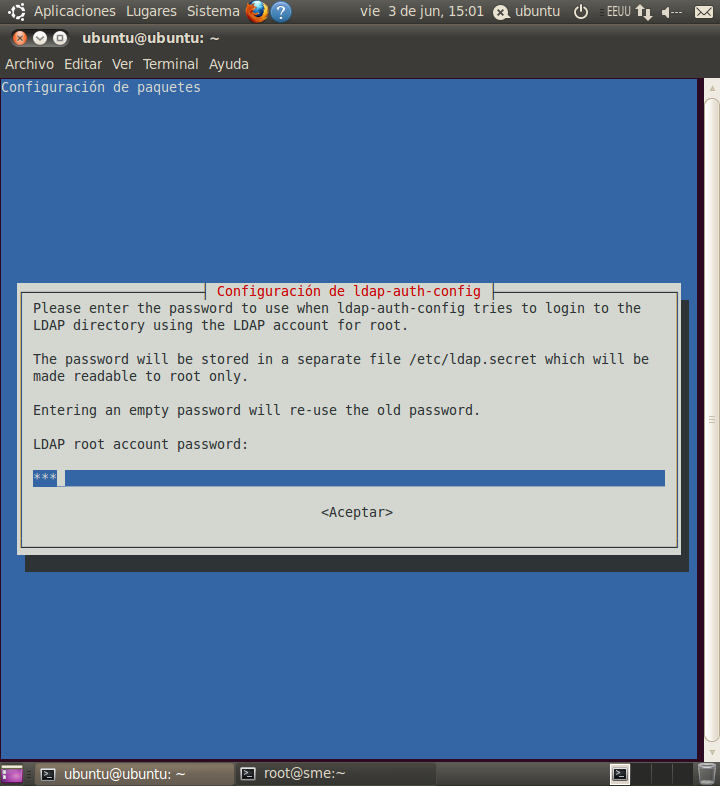
\includegraphics[width=\textwidth]{firewall/23.png}
\end{figure}

%\begin{longtable}{p{0.21\textwidth} | p{0.7\textwidth}}
%\textbf{Parámetro} & \textbf{Descripción}\\\hline
%\end{longtable}

%BIBLIOGRAFIAA
%https://wiki.contribs.org/Firewall
%http://blog.desdelinux.net/ddos-y-otros-ataques-vs-iptables-seguridad-anti-ddos-en-iptables/
%http://es.tldp.org/Manuales-LuCAS/GARL2/garl2/index.html
%http://www.cyberciti.biz/tips/linux-iptables-examples.html

